\section{Results}\label{sec:results}
The learning curves in Figure~\ref{fig:dshift_offline_normal} show the
$Q$-values evolution for the proposed agents as a result of offline
training.

% Q estimates discussion for:
% DQN offline
% NOTE why no BE on acrobot for DQN offline? maybe the env is too easy
% TODO say something about acrobot too, where no BE seems to occur...
The experiments confirmed previous findings for Q-learning
based agents when run offline on continuous domain problems: the $Q$
function incurs in a heavy overestimation bias produced by
bootstrapping errors. This is most evident on the \texttt{CartPole-v1}
environment, where DQN's $Q$-value estimates quickly escalate above
the true value. Since it has no access to ground truth values due to
the lack of exploration in the offline setting, the agent cannot
adjust the $Q$ function estimates while learning and the whole
estimation process diverges
\citep{pmlr-v97-fujimoto19a,kumar2019stabilizing}.

% DQV offline
% NOTE why dqv high BE or OB but still good performance on DQV?!
% motivate
% NOTE also, how is it possible that an on-policy algo is able to learn
% from off-policy data? answers: maybe does good imitation/only the V
% function is used for the TD-target
Among the studied algorithms, offline DQV is the most robust to the
bootstrapping error. On the \texttt{CartPole-v1} environment it is
almost able to correctly estimate the true value of $s_0$ for each
episode, consistently assessing at approximately $-10$ points from the
true solution. However, on the \texttt{Acrobot-v1} problem, offline
DQV still suffers from (stable) overestimation, although being the
algorithm which comes closest to the true value estimate of
$s_0$. DQV is likely capable of resisting the bootstrapping error
because it is an \textit{on-policy} algorithm. Although it should
theoretically not be able to learn in the offline setting, its strong
performance compared to the other agents is probably due to efficient
usage of the large offline dataset, which enables it to learn on-policy
discovering effective behaviors in the data. Moreover, DQV forms its
TD-target using only the state-value function $V$, therefore it cannot
possibly base predictions on those out-of-distribution actions which
are responsible for bootstrapping errors.

% DQV-Max offline
Offline DQV-Max is also more resilient to the bootstrapping error than
offline DQN.\ On the \texttt{CartPole-v1} environment, it estimates
the true value for $s_0$ almost perfectly, showing no detrimental
effects due to misaligned bootstrap estimates. As it is the case for
offline DQV and DQN, it still overestimates the real $Q$-value for
$s_0$ on the \texttt{Acrobot-v1} problem, positioning in between the
estimates of DQN and DQV.\ The low $Q$-value estimates on the
\texttt{CartPole-v1} environment are most likely in virtue of
DQV-Max's decoupling of \textit{selection} and \textit{evaluation}.
DQV-Max forms its temporal difference regression targets (selection)
from a model different than the one it uses to estimate the value of
the current state or state-action pair
(evaluation). \citet{sabatelli2020deep} note that this makes DQV-Max
less prone to the overestimation bias in the online setting, and these
experiments confirm the same results for the offline one.

% say something about the positive learning that occurred, regardless
% of Q estimates
% NOTE refer to reward plots in appendix/reward tables if eventually
% any
Finally, it should be mentioned that every agent is able to
learn to solve the proposed classic control environments in the
offline setting.
% NOTE maybe this sentence is not even necessary
However, the reward signals for the
\texttt{CartPole-v1} environment are noisier compared to the ones for
\texttt{Acrobot-v1}; in fact, the online behavioral DQN agent also
produced more unstable learning curves on the former problem.







% TODO new visible plots, only with Q estimates - just mention that
% all algorithms learn effectively. If implementing this modification
% -> update references to this in the methods section too, and maybe
% add tables summarizing numerical findings
\begin{figure}[!tbp]
  \centering
  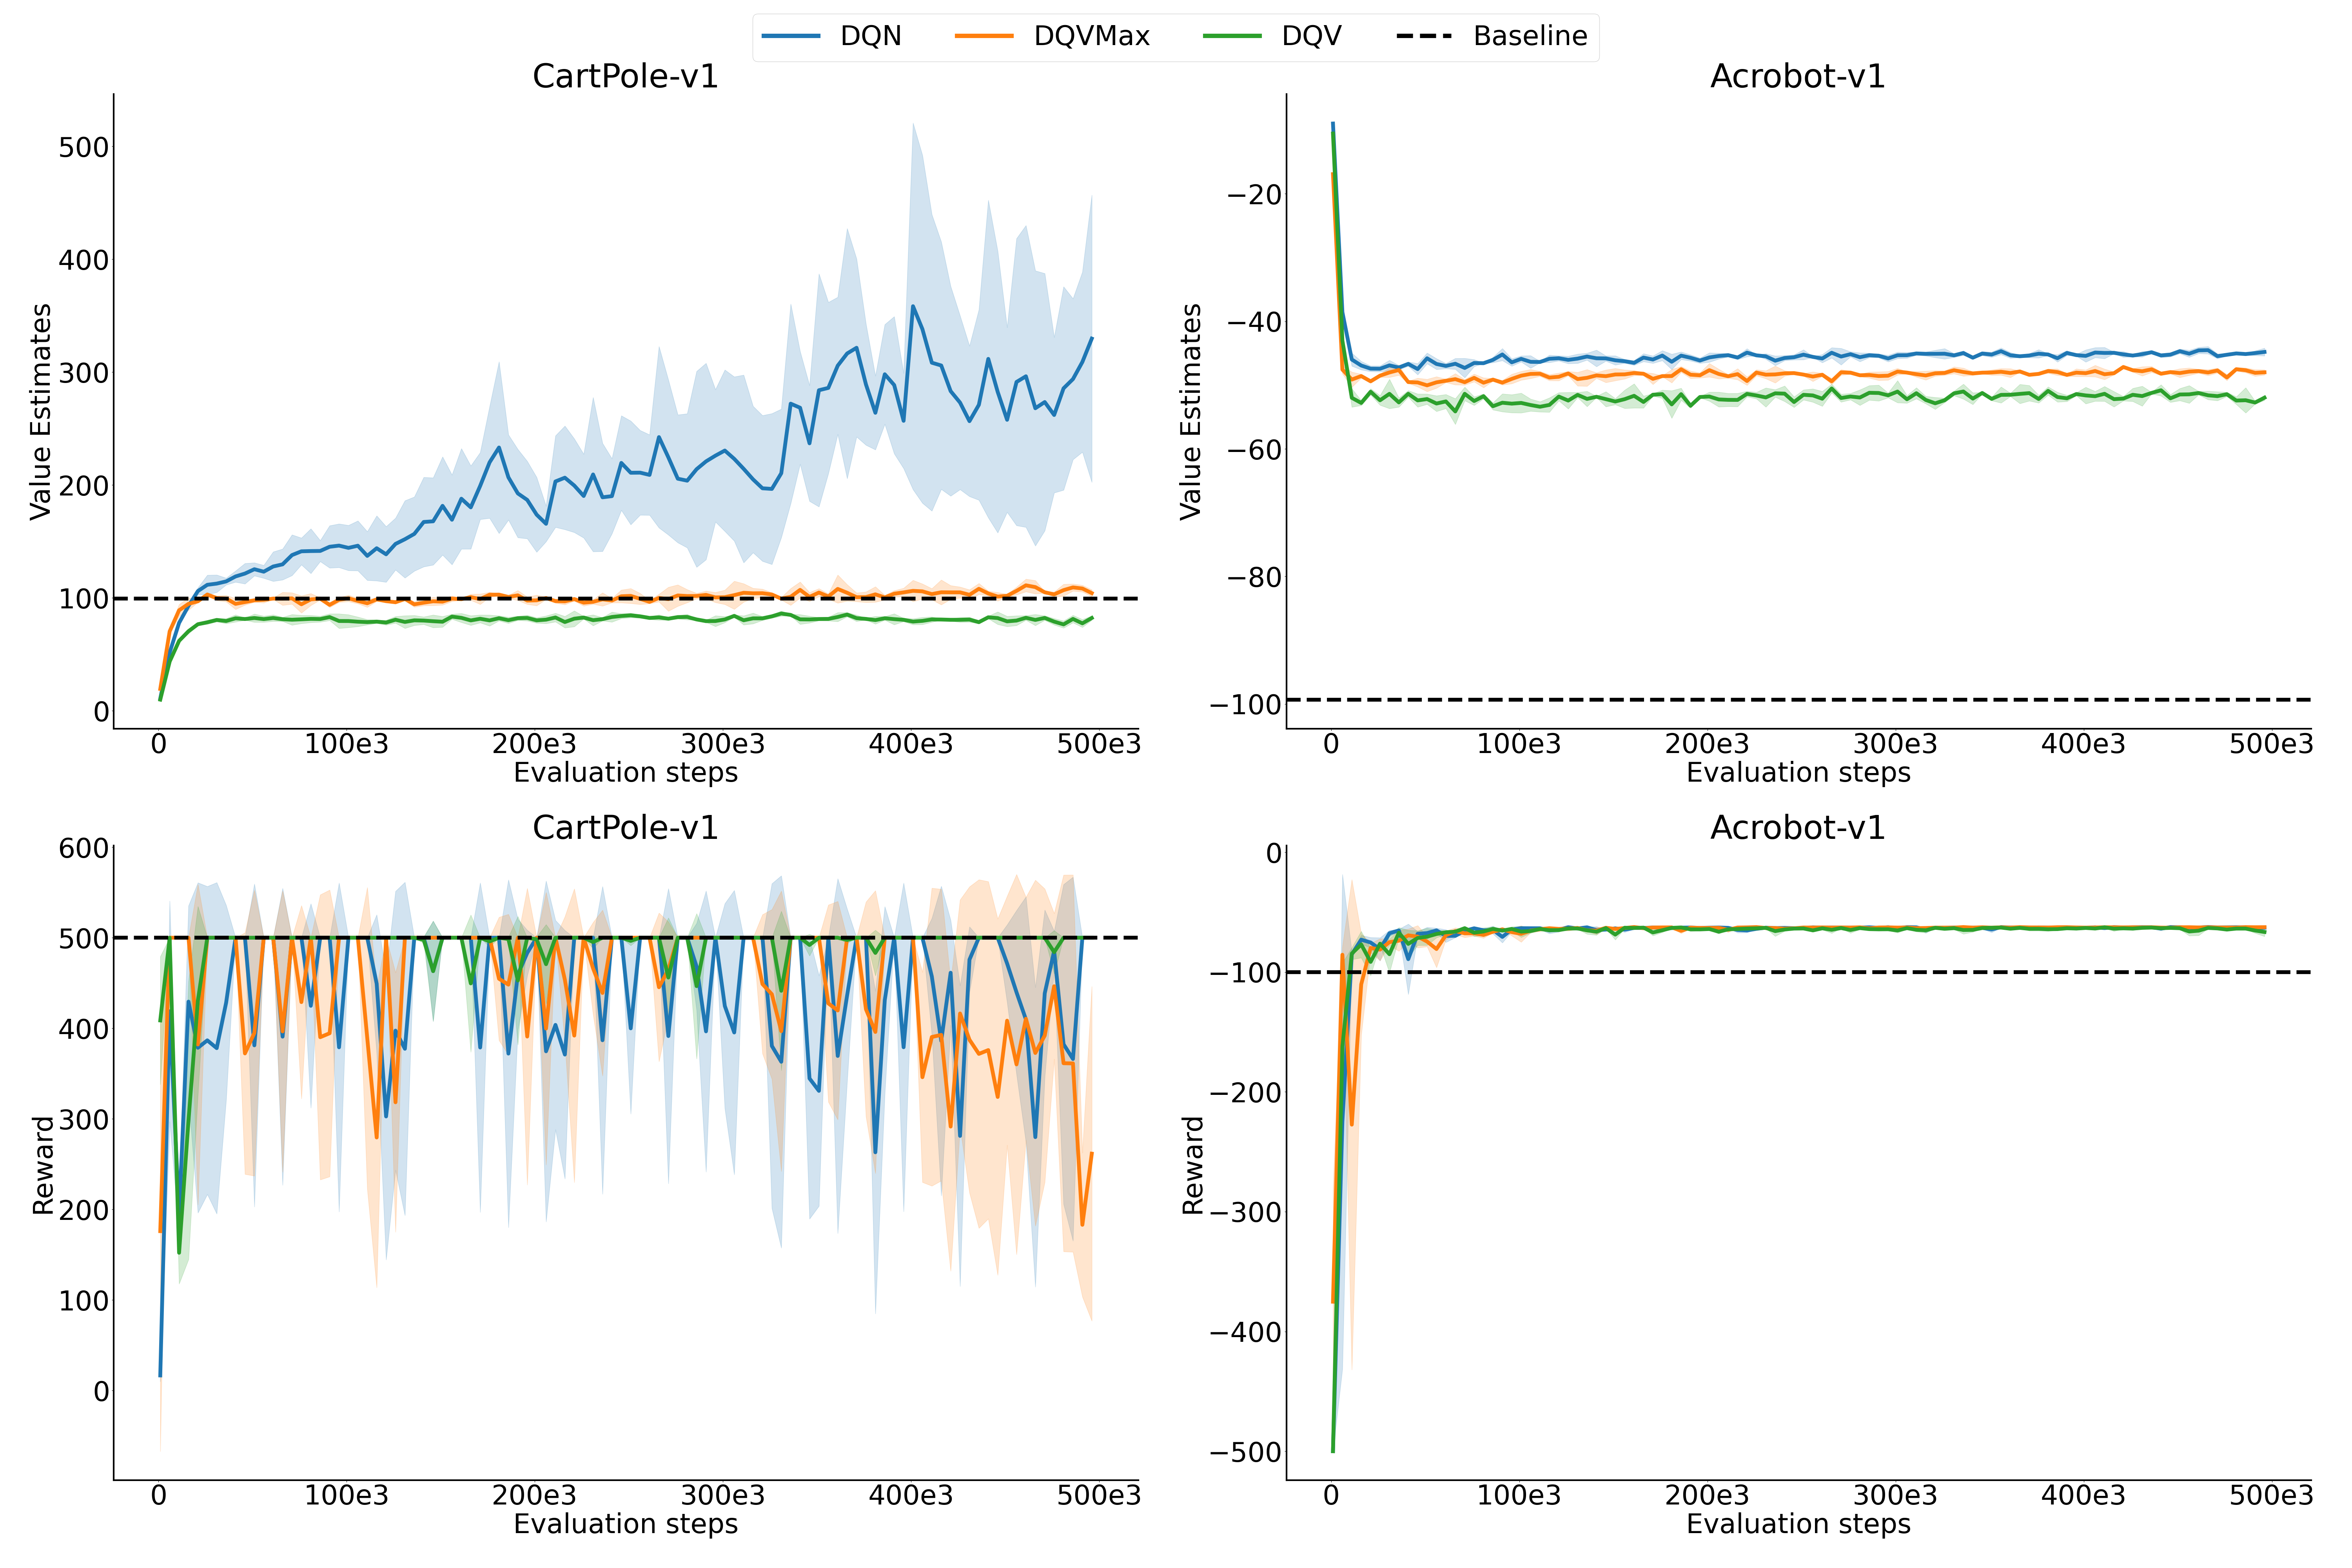
\includegraphics[width=.5\textwidth]{img/dshift_plots_normal.png}
  \caption{The $Q$-value estimates (top row) and actual return curves
    of offline DQN, DQV and DQV-Max at evaluation time. The shaded
    areas are $\pm$ 1 standard deviation from the mean of 3 different
    simulations.}\label{fig:dshift_offline_normal}
\end{figure}

\begin{figure}[!tbp]
  \centering
  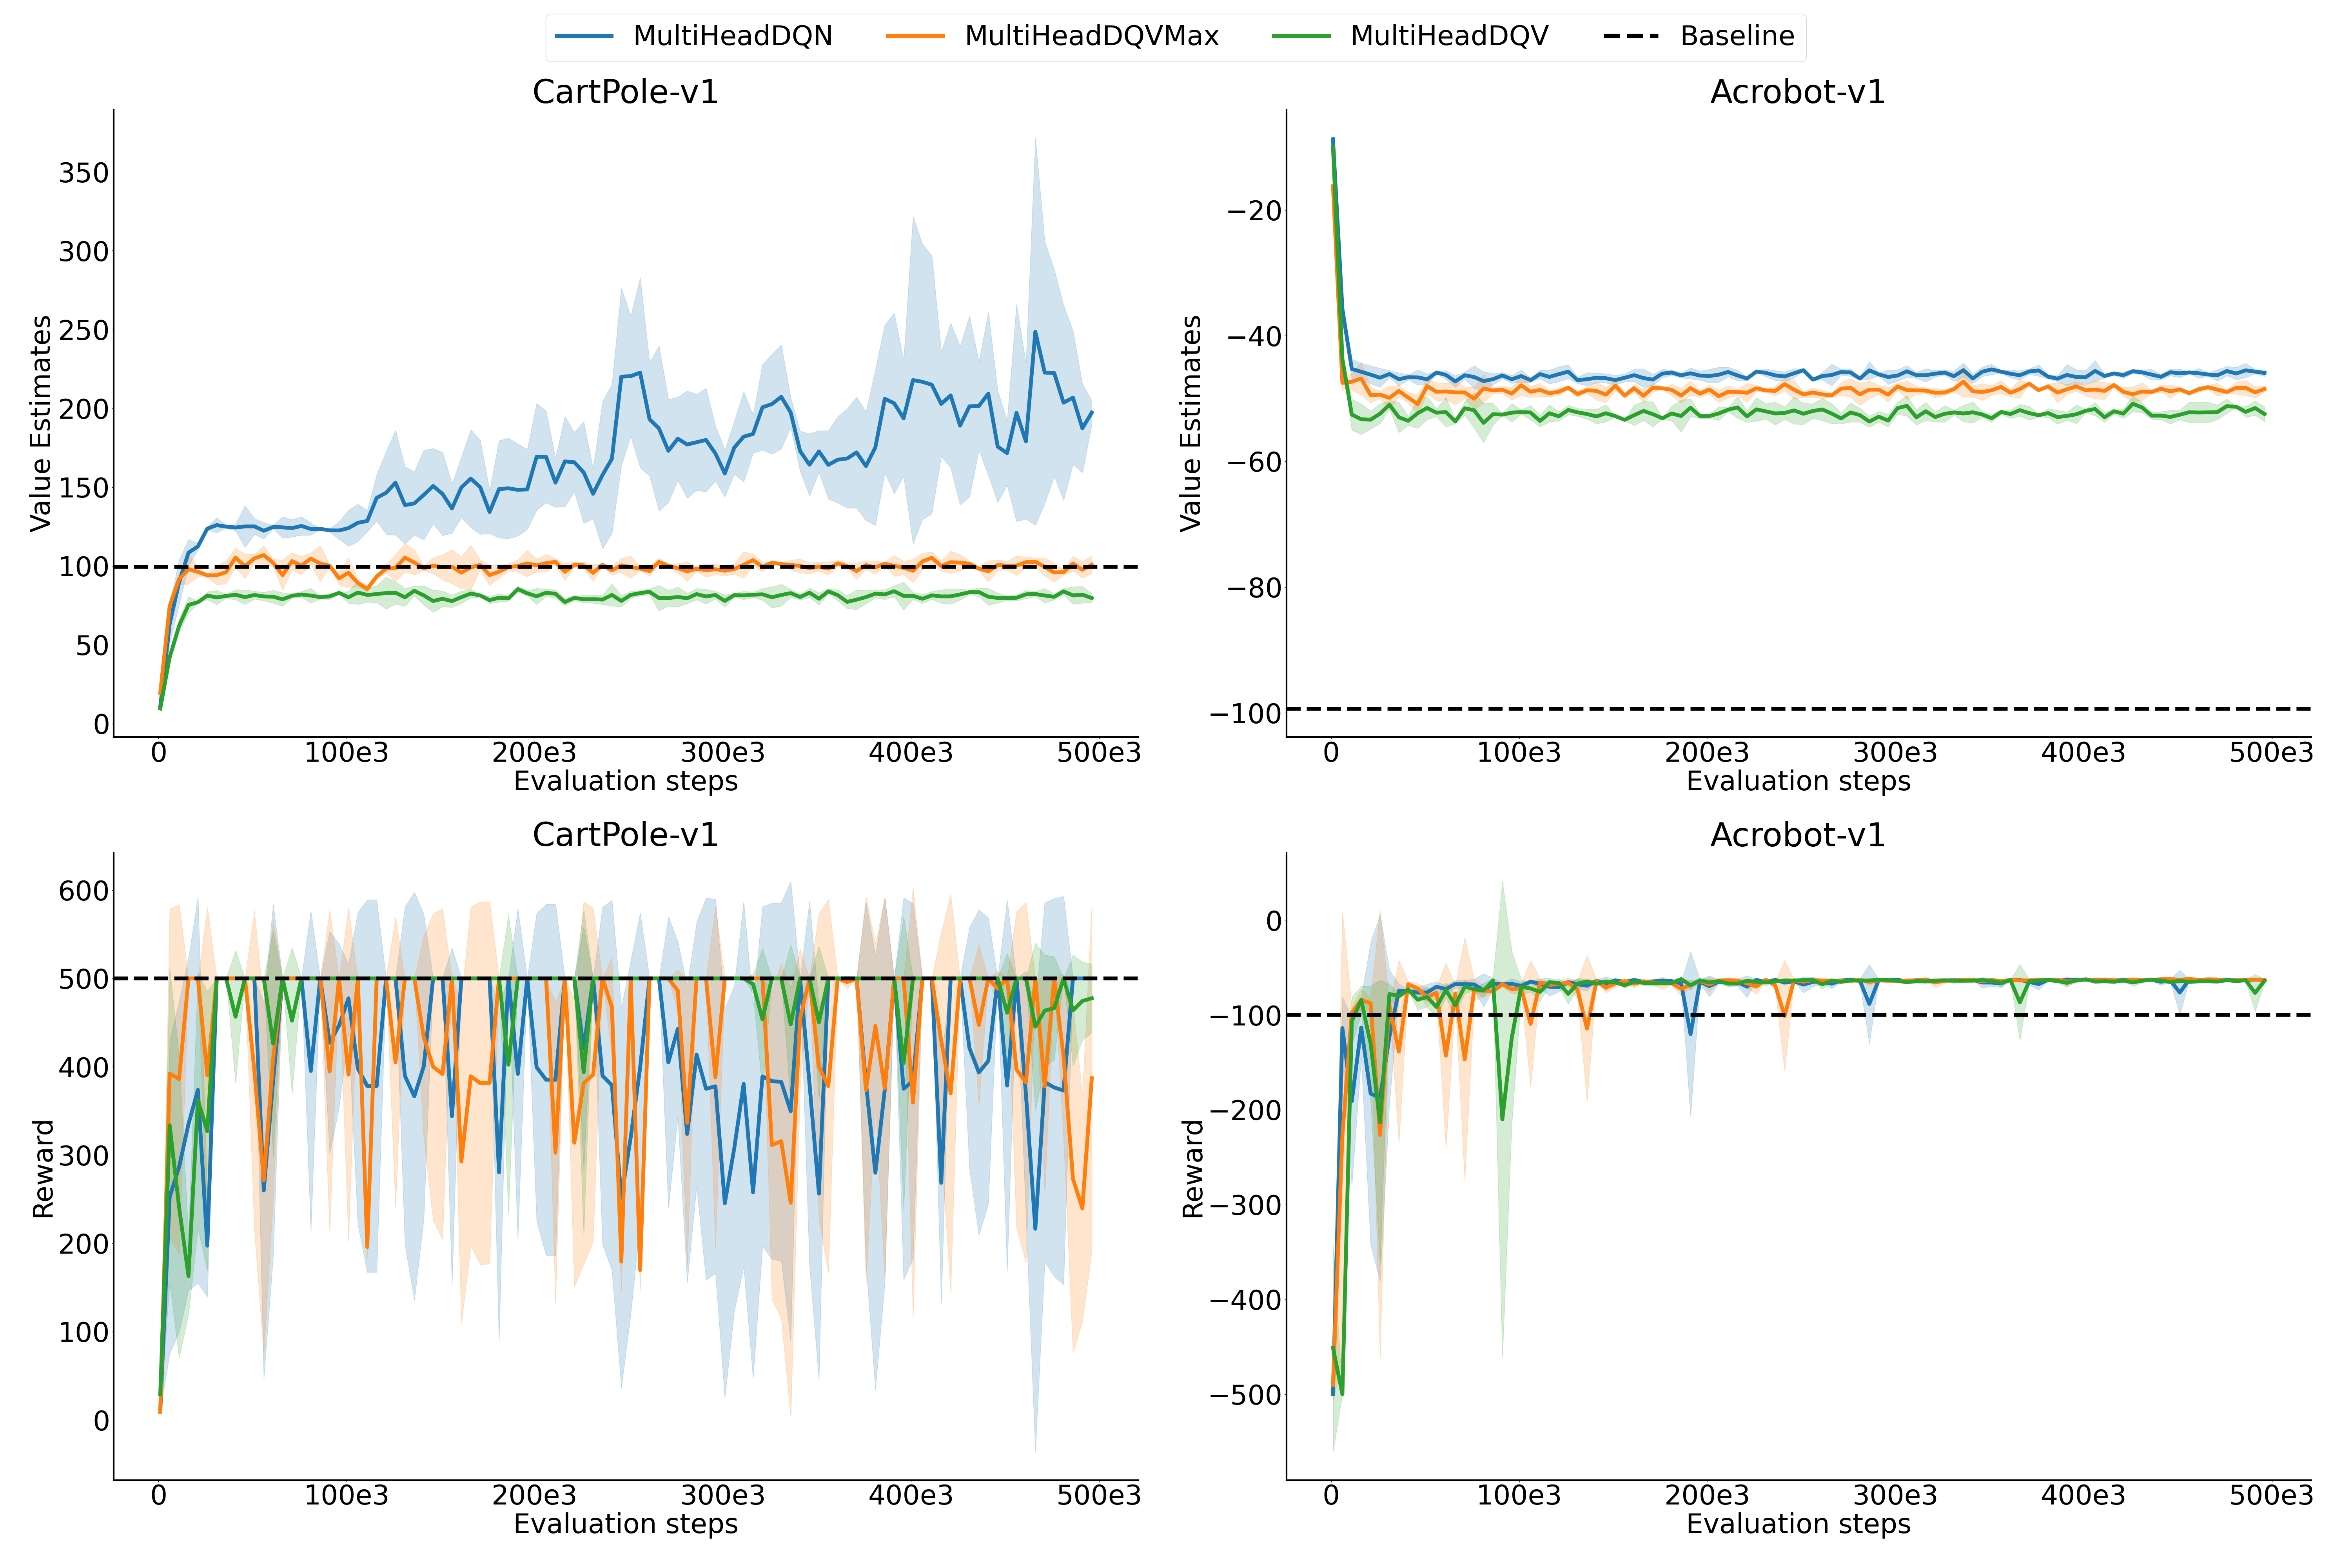
\includegraphics[width=.5\textwidth]{img/dshift_plots_ensembles.png}
  \caption{The $Q$-value estimates (top row) and actual return curves
    of offline DQN, DQV and DQV-Max at evaluation time. The shaded
    areas are $\pm$ 1 standard deviation from the mean of 3 different
    simulations.}\label{fig:dshift_offline_ensembles}
\end{figure}